\chapter{Functional design} \label{chap:func_design}
The functional design presents a high-level overview of the project and what explains what design choices were made on a system-level. Additionally, it provides tangential information that can be useful for understanding the working principle of the quantum sensing setup.

\section{Background knowledge}
Some background knowledge is required to understand the purpose of the projects, because the setup the project revolves around uses several non-trivial physics concepts. This section outlines the basic ideas behind the physics that enable the quantum sensing setup to work.

\subsection{Spin states}
Spin, at least in quantum mechanics, is the intrinsic angular momentum of a particle, which is described by the quantum number of the particle. Importantly, it differs from the angular momentum in classical mechanics, which is extrinsic. Spin characterizes systems of particles, usually electrons, using quantum entanglement. This phenomenon refers to the "entanglement", or spin correlation, of a set of particles.

These foundational concepts make it possible to describe quantum systems using various states. The most simple states, used as descriptors, are the energy states. Ground states refer to the system being in an energy minimum. On the other hand, excited states signify that the system has more energy than at its ground state. Additionally, there can be intermediate states during state transition.

While the aforementioned states describe system energy, they have no bearing on the spin. For the purposes of this project, only two spin states need to be explained. The first one is called singlet state. It occurs when an entangled system has a total spin of 0, caused by the mutual cancellation of spin. For example, for a system of two entangled electrons to be a singlet, the two spins would need to point in opposite directions. The second spin state is called triplet and it has a total spin of 1. Triplets can consist of, for instance, two unpaired electrons with aligned spins that sum up to 1. Singlets and triplets both have major distinguishing features and properties, which is why they can be used for quantum sensing. Aside from the difference in spin, triplets tend to have higher energy levels. They also exhibit attraction to magnetic fields, while singlets cannot be influenced directly by magnetism.

%\subsection{Energy levels and state transitions} and Zero-field splitting
\subsection{Zeeman effect}
Discovered by Pieter Zeeman in 1896, the Zeeman effect is another important phenomenon that enables quantum sensing. If under normal circumstances a light-emitting quantum system only emits one spectral line, then when a magnetic field is applied to it the line will split, thus exhibiting the Zeeman effect. In an \gls{nv} center, this phenomenon causes the $\ket{\pm1}$ energy level to split into $\ket{+1}$ and $\ket{-1}$. 

\subsection{Energy levels}\label{chap:energy_levels}
Figure \ref{fig:energylevels} shows the energy level diagram of an \gls{nv} center.
\begin{figure}[ht]
	\centering
	\includegraphics[width=0.7\linewidth]{img/energy_levels}
	\caption{\gls{nv} center energy level diagram (image credit to Song et al \cite{song2024enhancing})}
	\label{fig:energylevels}
\end{figure}

After illuminating the \gls{nv} center with a green laser, electrons go from a ground state to an excited state. They then need to return to the ground state. This decay process is usually direct and emits a red photon, however it can also go through the metastable singlet state and emit an infrared photon. It should be noted that whenever the \gls{nv} center is exposed to the resonant frequency $\nu = 2,87 GHz$ the probability of emitting an infrared photon is significantly increased.


\section{Quantum protocols}
There are a number of different quantum protocols, which differ in what they can measure, in how precisely they can measure it and in the complexity of the hardware they require to operate. \gls{cwodmr} is the main protocol this project is aimed at facilitating. As Saijo et al \cite{saijo2018ac} demonstrate, \gls{cwodmr} is relatively simple, while still detecting magnetic field with reasonable sensitivity. \gls{podmr} does outperform \gls{cwodmr} \cite{zhang2020high}, but because of the added complexity working with it is a "Could have" (see Chapter \ref{project_boundaries}). Before being able to run \gls{podmr} on the setup at the lab, several protocols need to be implemented first \cite{sewani2020coherent}. $T_1$ measurements, which are one of the fundamentals of \gls{mri}, should be conducted first. Afterwards, Rabi oscillations need to be observed and measured in order to calibrate the setup. Without these intermediate protocols, \gls{podmr} cannot be performed.



\subsection{\glsfmtshort{cwodmr}}
\gls{cwodmr} is a quantum protocol that has seen extensive usage in sensing setups that measure magnetic fields. Its working principle is centered around the photoluminescence of \gls{nv} centers and the difference in light emission based on spin states. As already discussed in Chapter \ref{chap:energy_levels}, the \gls{nv} center emits less visible light when at the resonant frequency $\nu$. Additionally, two more dips appear on the spectrum if a magnetic field is applied.Calculating the magnetic field can be done using the formula $h\nu = g_e\mu_BB_{AC}$ \footcite[In the formula, $h$ is the Planck constant, $g_e$ is the g-factor of the electron and $\mu_B$ is the Bohr magneton. Knowing all other variables, $B_{AC}$ can easily be calculated.]{enwiki:1301371272}. Figure \ref{fig:cwodmr} shows an example of what a \gls{cwodmr} spectrum might look like. 

\begin{figure}[ht]
	\centering
	\includegraphics[width=0.7\linewidth]{img/cw_odmr}
	\caption{Example of a \gls{cwodmr} spectrum \textbf{\textcolor{red}{with}} and \textbf{without} a magnetic field (image credit Saijo et al \cite{saijo2018ac})}
	\label{fig:cwodmr}
\end{figure}


\subsection{$T_1$ relaxometry}\label{chap:fd:t1}
$T_1$, $T_2$ and $T_2^*$ relaxation time measurements are commonly associated with radiometry \cite{ballinger23}, but they have other uses too. $T_1$ measurements, in particular, are useful in the realm of quantum sensing. Knowing the $T_1$ relaxation time, which refers to the time it takes for the spins in an \gls{nv} system to decay back to their original state, makes it possible to adjust the pulse sequences of more complex protocols and thus get better results.  %explain what relaxation is and the protcol

% % alternative to tikz diagram
%\begin{figure}[ht]
%	\centering
%	\includegraphics[width=0.9\linewidth]{drawio_diagrams/t1_waveforms.drawio}
%	\caption{Laser and reference signals for $T_1$ measurements}
%	\label{fig:t1waveforms}
%\end{figure}

\begin{figure}[ht]
	\centering
	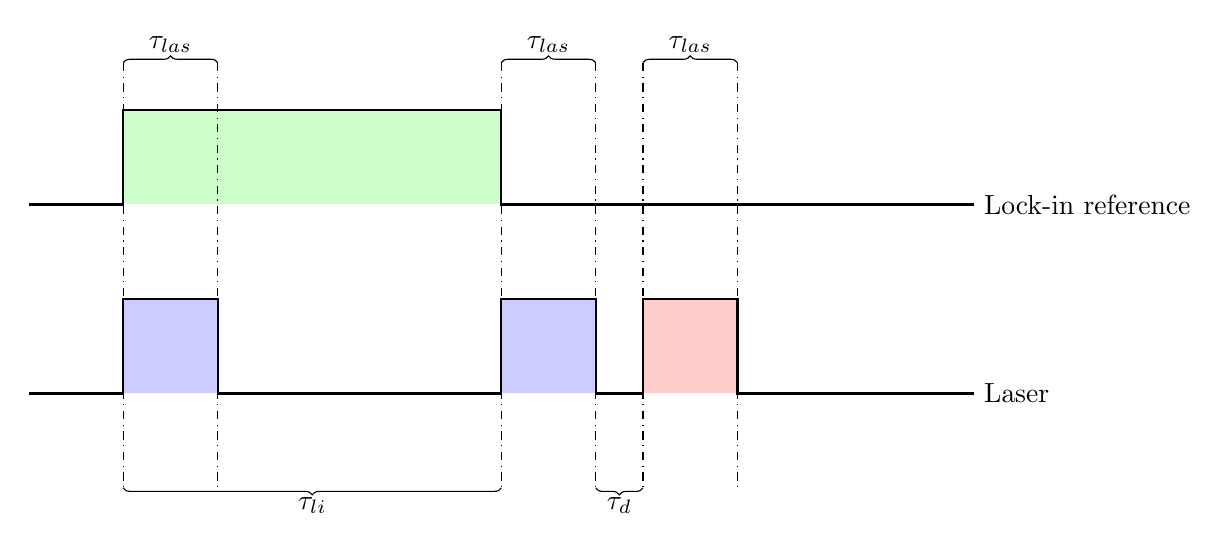
\begin{tikzpicture}[scale=.3]
		% TTL signal rectangles
		\fill [blue!20] 		(4,0) 	rectangle (8,4);
		\fill [blue!20] 		(20,0) 	rectangle (24,4);
		\fill [red!20]			(26,0)	rectangle (30,4);
		\fill [green!20] 		(4,8) 	rectangle (20,12);
		
		% signal lines
		\draw [thick] (0,0) -- (4, 0) -- (4,4) --(8,4) -- (8,0) -- (20,0) -- (20,4) -- (24,4) --(24,0) -- (26,0) -- (26,4) -- (30,4) -- (30,0) -- (40,0) node[anchor=west]{Laser};
		\draw [thick] (0,8) -- (4,8) -- (4,12) -- (20,12) -- (20,8) -- (40,8) node[anchor=west]{Lock-in reference}; % ref
		
		% curly braces top
		\draw [decorate, decoration={brace}] (4,14) -- (8,14) node[midway, above]{$\tau_{las}$};
		\draw [decorate, decoration={brace}] (20,14) -- (24,14) node[midway, above]{$\tau_{las}$};
		\draw [decorate, decoration={brace}] (26,14) -- (30,14) node[midway, above]{$\tau_{las}$};
		
		% curly braces bottom
		\draw [decorate, decoration={brace, mirror}] (4,-4) -- (20,-4) node[midway, below]{$\tau_{li}$};
		\draw [decorate, decoration={brace, mirror}] (24,-4) -- (26,-4) node[midway, below]{$\tau_{d}$};
		
		% dash-dotted lines
		\draw [dash dot] (4,14) -- (4,-4);
		\draw [dash dot] (8,14) -- (8,-4);
		\draw [dash dot] (20,14) -- (20,-4);
		\draw [dash dot] (24,14) -- (24,-4);
		\draw [dash dot] (26,14) -- (26,-4);
		\draw [dash dot] (30,14) -- (30,-4);
		
	\end{tikzpicture}
	\caption{Laser and reference signals for $T_1$ measurements}
	\label{fig:t1waveforms}
\end{figure}





The waveforms which are needed for $T_1$ measurements are shown if Figure \ref{fig:t1waveforms}. While both are important in practice, the lock-in is not as relevant, at least in this section of the report. However, its working principle is explored in Chapter \ref{chap:lockin}. For now, all that needs to be said about the lock-in reference signal is that it is periodic and $\tau_{li}$ is much longer than $\tau_{las}$ (Sewani et al \cite{sewani2020coherent} propose $\tau_{li} = 15 ms$ and $\tau_{las} = 5 \mu s$). Laser pulses, on the other hand, are not periodic. Instead, there are three short pulses every reference period (which is $2\tau_{li} s$ long). The two blue pulses have the same timing every cycle, because they initialize the \gls{nv} spins. However, the red pulse always occurs after the variable dark time $\tau_d$. Depending on the $T_1$ decay at the time of the readout pulse, a different voltage will be detected. Figure \ref{fig:t1result} shows what results can be expected when measuring $T_1$. Determining the value of $T_1$ is done using Formula \ref{eq:t1}, where $I$ is the light intensity, $I_\infty$ is the light intensity offset and $\tau_d$ is the dark time. 

\begin{equation}\label{eq:t1}
I(t)=I_\infty+I(0)e^{-\tau_d/T_1}
\end{equation}



\begin{figure}[ht]
	\centering
	\includegraphics[width=0.7\linewidth]{img/t1_result}
	\caption{Results of a set of $T_1$ measurements with varied dark time $\tau_d$ (image credit to Sewani et al \cite{sewani2020coherent})}
	\label{fig:t1result}
\end{figure}



\subsection{Other pulsed protocols}
There are several protocols which fall under the \gls{podmr} umbrella. Aside from $T_1$ measurements, Ramsey interferometry, Hahn echo and Rabi oscillations are the most common pulsed protocols. Supporting Rabi oscillations is the ultimate goal of the quantum sensing setup at the Applied Nanotechnology research group.

%todo_podmr: Finish Rabi explanation

\section{Quantum sensing setup}\label{chap:td:quantum_setup}
Executing all of the aforementioned protocols requires a sensing setup with some specific capabilities. This section discusses the devices that make up the setup and the functionalities require by each protocol.

A high-level diagram of the quantum sensing system can be seen in Figure \ref{fig:overview_high_lvl}. There are 2 input devices in the system, but most protocols exclusively use the function generator. On the other hand, only a single lock-in amplifier is used as an output device for all measurements. 

The blue boxes show the components responsible for sending and receiving light signals. They constitute the core of the setup. Waveforms are generated by the function generator, no matter the protocol. Using a current driver, the laser is then used to illuminate the diamond sample. The resulting luminescence is then measured by the photodetector and processed by the lock-in amplifier. All protocols need this part of the setup, however they utilize it differently.

Microwave generation, when needed, starts with a \gls{ttl} signal from the function generator or a frequency sweep using a dedicated device. Out of all protocols, only \gls{cwodmr} requires a sweep. The antenna then broadcasts the signal, while the switch isolates the signal generator from it. 


% Thorlabs Photodiodes and Photoconductors Tutorial:
% https://www.thorlabs.com/newgrouppage9.cfm?objectgroup_id=9020
\section{Laser driver}
As discussed in Chapter \ref{specifications}, the laser driver has already been designed and built. It gets \gls{ttl} signals from a waveform generator and outputs current to drive the connected laser.

However, the designer explicitly states that tests were only done with frequencies of up to 100 \unit{\kilo\hertz} \cite{sitnic2023}. This is insufficient for the project, as for example, the pulsing sequence for $T_1$ measurements use pulses with duration of 5 \unit{\micro\second} and downtime of as little as 1 \unit{\micro\second}\footnote{These values are taken from Sewani et al \cite{sewani2020coherent}, but the clients wants to make the timings used by the quantum sensing setup even faster}.


\section{Photodetection}
Photodetection is how the \gls{nv} photoluminescence is measured, effectively turning light into current using a photodiode. However, a bare photodiode cannot be connected to a lock-in amplifier, because it functions as a current generator. This is where the photodetection \gls {pcb} comes in. Its purpose is to transform the current into voltage and then amplify the resulting signal to the necessary voltage level. 

\subsection{Photodiodes}\label{chap:fd:photodiodes}
At the heart of the photodetector lies the photodiode. It is what turns light into current and drives the \gls{tia} that follows it. The specifications of the diode are an important part of the photodetector circuit. Photodiode biasing is another vital aspect of the photodetector, as it dictates the noise levels and bandwidth, thus directly influencing the amplifier design.

\begin{figure}[ht]
	\centering
	\includegraphics[width=0.5\linewidth]{img/bpw34_sens}
	\caption{BPW34 sensitivity (image credit to the BPW34 documentation \cite{vishay2011bpw34})}
	\label{fig:fd:bpw34sens}
\end{figure}



\begin{figure}[ht]
	\centering
	\begin{subfigure}[1a]{.49\linewidth}
		\begin{circuitikz}
			\tikzstyle{every node}=[font=\normalsize]
			\draw [ line width=0.5pt](3.75,9) to[empty photodiode,l={ \normalsize $D_1$}] (3.75,10.75);
			\draw [ line width=0.5pt](6.5,10.25) node[op amp,scale=1] (opamp2) {};
			\draw [ line width=0.5pt](opamp2.+) to[short] (5,9.75);
			\draw [ line width=0.5pt] (opamp2.-) to[short] (5,10.75);
			\draw [ line width=0.5pt](7.7,10.25) to[short](8,10.25);
			\draw [line width=0.5pt](5,9) to (5,8.25) node[ground]{};
			\draw [ line width=0.5pt](5,8.5) to[short] (5,9.75);
			\draw [ line width=0.5pt](3.75,10.5) to[short] (3.75,10.75);
			\draw [ line width=0.5pt](3.75,10.75) to[short] (5,10.75);
			\node at (4.5,10.75) [circ] {};
			\draw [ line width=0.5pt](4.5,10.75) to[short] (4.5,13.5);
			\draw [ line width=0.5pt](4.5,12.25) to[short] (5,12.25);
			\draw [ line width=0.5pt](4.5,13.5) to[short] (5,13.5);
			\draw [ line width=0.5pt](7.5,10.25) to[short] (7.5,11);
			\draw [ line width=0.5pt](5,12.25) to[european resistor,l={ \normalsize $R_1$}] (7,12.25);
			\node at (4.5,12.25) [circ] {};
			\draw [ line width=0.5pt](7,12.25) to[short] (7.5,12.25);
			\draw [ line width=0.5pt](7.5,12.25) to[short] (7.5,11);
			\draw [ line width=0.5pt](7.5,12.25) to[short] (7.5,13.5);
			\draw [line width=0.5pt](5,13.5) to[C,l={ \normalsize $C_1$}] (7,13.5);
			\node at (7.5,12.25) [circ] {};
			\draw [ line width=0.5pt](7,13.5) to[short] (7.5,13.5);
			\draw [ line width=0.5pt](8,10.25) to[short, -o] (8.25,10.25) node {$\ \ \ \ \ \ \ \ \ V_{out}$};
			\draw [ line width=0.5pt](3.75,10.75) to[short] (3.75,10.5);
			\draw [line width=0.5pt](3.75,9) to [short, -o] (3.75,8.25) node{$\ \ \ \ \ \ \ \ \ V_{EE}$};
			\draw [ dashed] (3,8) rectangle  (4.75,11);
		\end{circuitikz}
		\caption{Photoconductive mode}
		\label{fig:fd:biasing:pc}
	\end{subfigure}
	\hfill
	\begin{subfigure}[1b]{.49\linewidth}
		\begin{circuitikz}
			\tikzstyle{every node}=[font=\normalsize]
			\draw [ line width=0.5pt](3.75,9) to[empty photodiode,l={ \normalsize $D_1$}] (3.75,10.75);
			\draw [ line width=0.5pt](6.5,10.25) node[op amp,scale=1] (opamp2) {};
			\draw [ line width=0.5pt](opamp2.+) to[short] (5,9.75);
			\draw [ line width=0.5pt] (opamp2.-) to[short] (5,10.75);
			\draw [ line width=0.5pt](7.7,10.25) to[short](8,10.25);
			\draw [line width=0.5pt](5,9) to (5,8.25) node[ground]{};
			\draw [ line width=0.5pt](5,8.5) to[short] (5,9.75);
			\draw [ line width=0.5pt](3.75,10.5) to[short] (3.75,10.75);
			\draw [ line width=0.5pt](3.75,10.75) to[short] (5,10.75);
			\node at (4.5,10.75) [circ] {};
			\draw [ line width=0.5pt](4.5,10.75) to[short] (4.5,13.5);
			\draw [ line width=0.5pt](4.5,12.25) to[short] (5,12.25);
			\draw [ line width=0.5pt](4.5,13.5) to[short] (5,13.5);
			\draw [ line width=0.5pt](7.5,10.25) to[short] (7.5,11);
			\draw [ line width=0.5pt](5,12.25) to[european resistor,l={ \normalsize $R_1$}] (7,12.25);
			\node at (4.5,12.25) [circ] {};
			\draw [ line width=0.5pt](7,12.25) to[short] (7.5,12.25);
			\draw [ line width=0.5pt](7.5,12.25) to[short] (7.5,11);
			\draw [ line width=0.5pt](7.5,12.25) to[short] (7.5,13.5);
			\draw [line width=0.5pt](5,13.5) to[C,l={ \normalsize $C_1$}] (7,13.5);
			\node at (7.5,12.25) [circ] {};
			\draw [ line width=0.5pt](7,13.5) to[short] (7.5,13.5);
			\draw [ line width=0.5pt](8,10.25) to[short, -o] (8.25,10.25) node {$\ \ \ \ \ \ \ \ \ V_{out}$};
			\draw [ line width=0.5pt](3.75,10.75) to[short] (3.75,10.5);
			\draw [line width=0.5pt](3.75,9) to (3.75,8.25) node[ground]{};
			\draw [ dashed] (3,7.5) rectangle  (4.25,11);
		\end{circuitikz}
		\caption{Photovoltaic mode}
		\label{fig:fd:biasing:pv}
	\end{subfigure}
	\caption{Photodiode modes in a photodetector circuit}
	\label{fig:fd:biasing}
\end{figure}

Figure \ref{fig:fd:bpw34sens} shows the sensitivity of the BPW34, which is the diode used in the setup. The green laser that is used to excite the \gls{nv} centers has a wavelength of 550 \unit{\nano\meter}. On the other hand, the light emitted from the \gls{nv} centers has a wavelength of \numrange{637}{800} \unit{\nano\meter}, which is near the most sensitive wavelength range of the sensor. Although green light is not detected as well as red and infrared light, the much higher intensity of the laser means that there is an optical low-pass filter required to measure the \gls{nv} center luminescence. After filtering, the client said they expected less than 50 \unit{\nano\ampere} of photocurrent output, which they wanted to be translated to \numrange{0}{5} \unit{\volt}.



The two most common photodiode modes when applied to photodetectors are shown in Figure \ref{fig:fd:biasing}. Reverse-biased circuits, similar to the one in Figure \ref{fig:fd:biasing:pc}, are used in optical receivers and other high-speed use cases. However, the drawback of biasing the diode using the negative supply voltage $V_{EE}$ is that it results in an increased dark current, which is current that, unlike photocurrent, runs through the diode without any light being present. In the case of the BPW34, that dark current can be up to 30 \unit{\nano\ampere}. That much current can render the amplified signal unreadable. Precise low-light measurements, such as those needed by the quantum setup, require the photodetector to have high linearity, which cannot be achieved when the dark current is comparable to the photocurrent. Photovoltaic-mode biasing reduces the dark current at the cost of signal strength and bandwidth \cite{photodiodephotodiode}. This configuration is much more common in low-illumination setups, where the signals can be in the nanoampere to picoampere range. As the photoluminescent \gls{nv} centers emit extremely low amounts of light, the photovoltaic configuration was chosen for the photodetector implementation for the quantum sensing setup. 



\subsection{\glsfmtshort{tia} design} \label{chap:photodetection_design}
Designing the photodetector is mostly about creating a \gls{tia}, which is a tool used for converting current to voltage, and specifically tuning its parameters so that it works with the selected photodiode under operating conditions. 

\begin{figure}[ht]
	\centering
	\resizebox{.5\textwidth}{!}{%
		\begin{circuitikz}
			\tikzstyle{every node}=[font=\normalsize]
			\draw [ line width=0.5pt](3.75,9) to[empty photodiode,l={ \normalsize $D_1$}] (3.75,10.75);
			\draw [ line width=0.5pt](6.5,10.25) node[op amp,scale=1] (opamp2) {};
			\draw [ line width=0.5pt](opamp2.+) to[short] (5,9.75);
			\draw [ line width=0.5pt] (opamp2.-) to[short] (5,10.75);
			\draw [ line width=0.5pt](7.7,10.25) to[short](8,10.25);
			\draw [line width=0.5pt](5,9) to (5,8.25) node[ground]{};
			\draw [ line width=0.5pt](5,8.5) to[short] (5,9.75);
			\draw [ line width=0.5pt](3.75,10.5) to[short] (3.75,10.75);
			\draw [ line width=0.5pt](3.75,10.75) to[short] (5,10.75);
			\node at (4.5,10.75) [circ] {};
			\draw [ line width=0.5pt](4.5,10.75) to[short] (4.5,13.5);
			\draw [ line width=0.5pt](4.5,12.25) to[short] (5,12.25);
			\draw [ line width=0.5pt](4.5,13.5) to[short] (5,13.5);
			\draw [ line width=0.5pt](7.5,10.25) to[short] (7.5,11);
			\draw [ line width=0.5pt](5,12.25) to[european resistor,l={ \normalsize $R_1$}] (7,12.25);
			\node at (4.5,12.25) [circ] {};
			\draw [ line width=0.5pt](7,12.25) to[short] (7.5,12.25);
			\draw [ line width=0.5pt](7.5,12.25) to[short] (7.5,11);
			\draw [ line width=0.5pt](7.5,12.25) to[short] (7.5,13.5);
			\draw [line width=0.5pt](5,13.5) to[C,l={ \normalsize $C_1$}] (7,13.5);
			\node at (7.5,12.25) [circ] {};
			\draw [ line width=0.5pt](7,13.5) to[short] (7.5,13.5);
			\draw [ line width=0.5pt](8,10.25) to[short, -o] (8.25,10.25) node {$\ \ \ \ \ \ \ \ \ V_{out}$};
			\draw [ line width=0.5pt](3.75,10.75) to[short] (3.75,10.5);
			\draw [line width=0.5pt](3.75,9) to (3.75,8.25) node[ground]{};
			\draw [line width=0.5pt, ->, >=Stealth] (4.25,9.25) -- (4.25,10.25);
			\node [font=\normalsize] at (4.60,9.75) {$I_f$};
		\end{circuitikz}
	}%
	\caption{Basic \gls{tia} circuit}
	\label{fig:tia}
\end{figure}

The basic circuit, shown in Figure \ref{fig:tia}, is all that is required for photodetection. Following the Texas Instruments guidelines for making a \gls{tia} \cite{semig24}, all the parameters of the circuit can be calculated.

\begin{equation}\label{eq:r1}
	R_1 = \frac{V_{o\ max}}{I_{f\ max}}\ \text{assuming}\ V_{o\ min} = 0 \unit{\volt}
\end{equation}

The resistor $R_1$ determines the transimpedance gain of the amplifier. Equation \eqref{eq:r1} shows how its value can be calculated by using the output voltage and input current. It should be noted that the minimum output voltage is always 0 in this use case.

\begin{equation}\label{eq:c1}
	C_1 = \frac{1}{2 \pi R_1 f_{rc}}
\end{equation}

The ideal capacitance of $C_1$ can be calculated using the resistance of $R_1$ and the cutoff frequency $f_{rc}$, as shown in Equation \eqref{eq:c1}. To select a physical capacitor based on the calculated value, its capacitance should be less than or equal to the ideal value.


In addition, a non-inverting amplifier can be added, to increase the gain of the circuit even more, without affecting the phase. Figure \ref{fig:tia_nia} shows how it can be connected to the output of the \gls{tia} from Figure \ref{fig:tia}.

\begin{figure}[ht]
	\centering
	\resizebox{.9\textwidth}{!}{%
		\begin{circuitikz}
			\tikzstyle{every node}=[font=\normalsize]
			\draw [ line width=0.5pt](3.75,9) to[empty photodiode,l={ \normalsize $D_1$}] (3.75,10.75);
			\draw [ line width=0.5pt](6.5,10.25) node[op amp,scale=1] (opamp2) {};
			\draw [ line width=0.5pt](opamp2.+) to[short] (5,9.75);
			\draw [ line width=0.5pt] (opamp2.-) to[short] (5,10.75);
			\draw [ line width=0.5pt](7.7,10.25) to[short](8,10.25);
			\draw [line width=0.5pt](5,9) to (5,8.25) node[ground]{};
			\draw [ line width=0.5pt](5,8.5) to[short] (5,9.75);
			\draw [ line width=0.5pt](3.75,10.5) to[short] (3.75,10.75);
			\draw [ line width=0.5pt](3.75,10.75) to[short] (5,10.75);
			\node at (4.5,10.75) [circ] {};
			\draw [ line width=0.5pt](4.5,10.75) to[short] (4.5,13.5);
			\draw [ line width=0.5pt](4.5,12.25) to[short] (5,12.25);
			\draw [ line width=0.5pt](4.5,13.5) to[short] (5,13.5);
			\draw [ line width=0.5pt](7.5,10.25) to[short] (7.5,11);
			\draw [ line width=0.5pt](5,12.25) to[european resistor,l={ \normalsize $R_1$}] (7,12.25);
			\node at (4.5,12.25) [circ] {};
			\draw [ line width=0.5pt](7,12.25) to[short] (7.5,12.25);
			\draw [ line width=0.5pt](7.5,12.25) to[short] (7.5,11);
			\draw [ line width=0.5pt](7.5,12.25) to[short] (7.5,13.5);
			\draw [line width=0.5pt](5,13.5) to[C,l={ \normalsize $C_1$}] (7,13.5);
			\node at (7.5,12.25) [circ] {};
			\draw [ line width=0.5pt](7,13.5) to[short] (7.5,13.5);
			\draw [ line width=0.5pt](3.75,10.75) to[short] (3.75,10.5);
			\draw [line width=0.5pt](3.75,9) to (3.75,8.25) node[ground]{};
			\draw [line width=0.5pt, ->, >=Stealth] (4.25,9.25) -- (4.25,10.25);
			\node [font=\normalsize] at (4.60,9.75) {$I_f$};
			\draw (8,10.25) to[short] (10.25,10.25);
			\draw (11.75,10.75) node[op amp,scale=1] (opamp2) {};
			\draw (opamp2.+) to[short] (10.25,10.25);
			\draw  (opamp2.-) to[short] (10.25,11.25);
			\draw (12.95,10.75) to[short](13.25,10.75);
			\draw (8.5,11.25) to[european resistor,l={ \normalsize $R_2$}] (10.25,11.25);
			\draw (8.5,11.25) to (8.5,11) node[ground]{};
			\draw (11.75,10.75) node[op amp,scale=1] (opamp2) {};
			\draw (opamp2.+) to[short] (10.25,10.25);
			\draw  (opamp2.-) to[short] (10.25,11.25);
			\draw (12.95,10.75) to[short](13.25,10.75);
			\node at (10.25,11.25) [circ] {};
			\draw (10.25,11.25) to[short] (10.25,12.5);
			\draw (10.25,12.5) to[european resistor,l={ \normalsize $R_3$}] (13,12.5);
			\draw (13,12.5) to[short] (13,10.75);
			\draw (13.25,10.75) to[short, -o] (13.5,10.75) node {$\ \ \ \ \ \ \ \ \ V_{out}$};
			\draw (13.5,10.75) to[short, -o] (13.5,10.75) ;
			\node at (7.5,10.25) [circ] {};
			\node [font=\normalsize, anchor=north] at (7.5,10.25) {$V_{ot}$};
			\node [font=\normalsize, anchor=north] at (10.5,11.25) {$V_{-}$};
		\end{circuitikz}
	}%
	\caption{\gls{tia} with non-inverting output amplification}
	\label{fig:tia_nia}
\end{figure}

Equation \eqref{eq:nia} is used to calculate the gain of second amplification stage. The formula is derived from the voltage divider formed by the two resistors and the fact that $V_{ot} = V_{-}$.

\begin{equation}\label{eq:nia}
	A_{nia} = \frac{V{out}}{V{ot}} = 1 + \frac{R_3}{R_2}
\end{equation}

The design is based on circuits provided by the client. At their request, the first version of the PCB is an exact replica of the original circuit.  

\subsection{Power requirements}\label{chap:fd:power_req}
Knowing the power needs of the photodetector is important for decreasing the size of the quantum setup. As bench power supplies take up a lot of space and exceed the photodetector requirements by orders of magnitude, an on-board supply or a breakout board will better fit the project. To minimize overhead while still having a supply that can handle the circuit, the power usage of the photodetector needs to be calculated. 

When calculating the power of the circuit in Figure \ref{fig:tia_nia}, the most important elements to consider are the op-amps. As the non-inverting amplifier has high input impedance, the system can be broken down into two op-amp circuits.

The op-amp in the \gls{tia} circuit has an intrinsic power dissipation caused by its quiescent current, as well as a load power dissipation. Due to the very high input impedance of the non-inverting topology that follows the \gls{tia}, there is no load current. Nevertheless, the feedback loop still draws a current $I_{f\alpha}$ from the amplifier. Equation \eqref{eq:fd:power:tia:current:fb} shows how this current can be calculated, after which the feedback power dissipation $I_{f\alpha}$ can be determined using Equation \eqref{eq:fd:power:tia:fb}. It should be noted that for $C_1R_1 \ll 1$ the equivalent impedance $Z_1$ is equivalent to the resistance $R_1$ at low frequencies.

\begin{equation}\label{eq:fd:power:tia:current:fb}
	\begin{cases}
		I_{f\alpha} = \frac{V_{ot}}{Z_1}\\
		Z_1 = R_1||(\frac{1}{sC_1}) = \frac{R_1}{1 + sC_1R_1}
	\end{cases}
\end{equation}

\begin{equation}\label{eq:fd:power:tia:fb}
	P_{f\alpha} = (V_{cc} - V_{ot})I_{f\alpha}
\end{equation}


As a characteristic of the amplifier \gls{ic}, the quiescent current $I_{q\alpha}$ can be taken from the datasheet to calculate its power dissipation $P_{q\alpha}$ with the formula shown in Equation \eqref{eq:fd:power:tia:q}.

\begin{equation}\label{eq:fd:power:tia:q}
	P_{q\alpha} = (V_{cc} - V_{ee})I_{q\alpha}
\end{equation}

Ultimately, the total power dissipation $P_{\alpha}$ of the \gls{tia} can be calculated by summing the results of the previous equations (see Equation \eqref{eq:fd:power:tia:total}).

\begin{equation}\label{eq:fd:power:tia:total}
	P_{\alpha} = P_{f\alpha} + P_{q\alpha}
\end{equation}

Similarly to the amplifier that was just discussed, the non-inverting op-amp has a quiescent power dissipation $P_{q\beta}$ and a load power dissipation $P_{f\beta}$. It should be noted that even though $V_out$ is not connected to in Figure \ref{fig:tia_nia}, the output of the photodetector in the sensing setup needs to be connected to a lock-in amplifier. Even then, the load current that runs through it is imperceptibly low, which is why the power in Equations \eqref{eq:fd:power:nia:current:fb} and \eqref{eq:fd:power:nia:fb} is calculated in a similar way. 

\begin{equation}\label{eq:fd:power:nia:current:fb}
		I_{f\beta} = \frac{V_{out} - V_{ot}}{R_3}\\
\end{equation}

\begin{equation}\label{eq:fd:power:nia:fb}
	P_{f\beta} = (V_{cc} - V_{out})I_{f\beta}
\end{equation}


Equation \eqref{eq:fd:power:nia:q} shows the quiescent power dissipation, which again is based on the intrinsic characteristics of the op-amp and combining all powers again yields the total power dissipation $P_\beta$ of the amplifier, shown in Equation \eqref{eq:fd:power:nia:total}.

\begin{equation}\label{eq:fd:power:nia:q}
	P_{q\beta} = (V_{cc} - V_{ee})I_{q\beta}
\end{equation}


\begin{equation}\label{eq:fd:power:nia:total}
	P_{\beta} = P_{f\beta} + P_{q\beta}
\end{equation}

Additionally, the power dissipated by $R_2$ is given in Equation \eqref{eq:fd:power:r2}.

\begin{equation}\label{eq:fd:power:r2}
	P_{2} = V_{ot}I_{f\beta}
\end{equation}

%\section{\glsfmtshort{olia} implementation}

\section{Lock-in amplification} \label{chap:lockin}
As a means of retrieving data, lock-in amplification is the most suitable for the setup due to its relatively low cost, signal retrieval capabilities and the possibility of using one amplifier for several setups. 

\begin{figure}[ht]
	\centering
	\includegraphics[width=0.7\linewidth]{img/lia_hl_schematic}
	\caption{High-level diagram of a lock-in amplifier (image credit to Zurich Instruments \cite{instruments2018principles})}
	\label{fig:liahlschematic}
\end{figure}

Figure \ref{fig:liahlschematic} shows an overview of how lock-in amplification works. Simply put, the amplifier receives a signal $V_s$ and extracts the data at the frequency of a reference signal $V_r$. To explain this more thoroughly, lock-in amplification utilizes the fact that every signal is made of periodic waves, which are equal to zero when averaged. 

\begin{equation}\label{eq:voltage_sig}
	V_s = R\cos{(\omega_st + \theta)} = \frac{R}{2}e^{i(\omega_st + \theta)} + \frac{R}{2}e^{-i(\omega_st + \theta)}
\end{equation}

Equation \eqref{eq:voltage_sig} shows how the mathematical expression of a sine wave signal, where $\omega_s$ is the frequency and $\theta$ is the phase of the signal. Using the trigonometric identity $\cos{x} = \frac{1}{2}(e^{ix} + e^{-ix})$, the signal can be represented in terms of complex numbers.

\begin{equation}\label{eq:voltage_ref}
	V_r = e^{-i\omega_rt}
\end{equation}

In Equation \eqref{eq:voltage_ref}, a simplified reference signal is shown. Real applications might require more complex reference signals, but $V_r$ is perfect for demonstrating the lock-in principle.

\begin{equation}\label{eq:voltage_mult}
	V_m = V_sV_r = \frac{R}{2}e^{i(\omega_s -\omega_r)t  + \theta} + \frac{R}{2}e^{-i(\omega_s +\omega_r)t + \theta}
\end{equation}

Finally, Equation \eqref{eq:voltage_mult} shows the product of the signal $V_s$ and the reference $V_r$. In the case of $\omega_s = \omega_r$, there is a signal at \num{0} \unit{\hertz} and another one at $2\omega_s$ \unit{\hertz}. The latter, however, should be attenuated to an undetectable level by the low-pass filters shown in Figure \ref{fig:liahlschematic}. This way, both the unwanted signal appearing at double the frequency and all of the noise at different frequencies is attenuated.


